\documentclass[main.tex]{subfiles}
\newcommand{\Break}{\State \textbf{break} }
\begin{document}

\chapter{基于随机森林的献血招募模型研究}

\section{献血者特征设计}
由于随机森林的输入必须为确定的特征的数值,包括离散值或者连续值。然而,
根据献血中心提供的原始数据来看,特征数目过于冗余,并且各个特征之间有的关联性
较强,有着互相依赖的关系。而且,一部分特征在某些献血者样本上存在数据缺失
值或错误值等问题,这给后续的模型设计与实验带来了一定的困扰与挑战,
所以,在数据挖掘领域中,常常需要特征提取的操作。献血者的特征提取设计,
可以看作是后续基于随机森林的献血招募模型的数据特征提取模块,它引入了
一些必要的专家知识,从而使得模型关注于对预测分类结果有直接或间接影响的
因素,并将降低减少这些特征之间的依赖关系,使得每个特征因素之间尽量是
独立的。再者,通过一些简单的数据预处理工作,也使得输入的样本数据分布
更加平衡,有助于从外部因素的角度,来进一步地提升模型的性能。

血液中心通常使用的短信招募献血人员的方法如图\ref{text_recruit}
所示,主要通过从近一年的
献血对象中,选择年龄不超过60岁且献血间隔达到6个月以上的,这部分对象由
于近期参与过献血活动,所以表明其在近期有献血意愿,是合理的潜在招募目标,
所以献血时间是一个对于是否参与献血的一个有效且极为重要的特征。同时,根据血液中心
以往招募献血的经验,发现职业与受教育程度对于一个人员是否来献血也是
十分重要的。表\ref{donate_record_1},\ref{donate_record_2}
和\ref{donate_record_3}显示了某个献血人员的一次献血记录,该表包含了个人的一些
基本特征,如年龄、性别、居住情况、是否有献血反应等,这些个人献血的基本信息
也存在影响个人献血的情况。可以看出,有的特征显然对最终血样合格与否没有
过多的影响,比如献血方式。另外也注意到,考虑到献血者的隐私保护问题,
有些特征是存在缺失值的,比如居住类型、工作组等。
更进一步地,原始数据中,往往一位献血者由于会多次献血,所以一个献血者
往往会在数据库中对应多条献血记录。如何充分挖掘并利用这个信息,是特征
提取的关键所在。经过初步的研究后发现,献血人员的献血意愿不
仅取决于一次献血,常常与其多次献血的记录有关,如献血次数、总献血量、
献血次数、献血频率等。根据经验与实验研究相结合,设计出包含年龄、性别、
血型、最近献血量、总献血量、献血次数、献血间隔、献血频率、血液检测是否
合格、教育程度、居住状态、职业、献血反应13项的特征库,
其中献血频率采用\ref{donate_freq}进行计算。

\begin{table*}[htbp!]
    \caption{某献血人员的献血记录}
    \label{donate_record_1}
    \centering
    \begin{tabular}{cccccccc}
    \hline
    献血者表示码   & 登记时间       & 献血量 & 采血时间       & 献血地点 & 血型 & Rh血型  & 性别  \\ \hline
    00****09 & 2000-07-22 & 200 & 2000-07-22 & 站内   & B  & **D** & 女 \\ \hline
    \end{tabular}
\end{table*}

\begin{table*}[htbp!]
    \caption{某献血人员的献血记录(续表\ref{donate_record_1})}
    \label{donate_record_2}
    \centering
    \begin{tabular}{ccccccc}
    \hline
    出生日期       & 国籍 & 民族 & 居住类型 & 职业 & 文化程度 & 所属区县 \\ \hline
    1974-11-19 & 中国 & 汉族 &      & 其他 & 其他   & 扬州市  \\ \hline
    \end{tabular}
\end{table*}

\begin{table*}[htbp!]
    \caption{某献血人员的献血记录(续表\ref{donate_record_1})}
    \label{donate_record_3}
    \centering
    \begin{tabular}{ccccccc}
    \hline
    工作组 & 实际采血量 & 检验结论 & 献血方式 & 采血类型 & 有非标量 & 是否有献血反应 \\ \hline
        & 200   & 合格   & 无偿   & 全血   & 标量   & 无       \\ \hline
    \end{tabular}
\end{table*}

\begin{equation}
    \label{donate_freq}
    \text{献血频率} = \frac{\text { 最近一次献血时间 } - \text {初次献血时间}}{\text {献血次数}}
\end{equation}


\begin{figure}[htbp!]
    \centering \includegraphics[width=0.6\textwidth]{img/zhaomu.png} 
    \caption{血液中心进行短信招募献血人员的方法示意图}
    \label{text_recruit}
\end{figure}

献血记录往往存在一定的缺失值,比如教育程度缺失、职业缺失等,为了处理这
一情况,采用了默认值代替缺失值,因此缺失教育程度使用初中及以下教育程度代替,
缺失职业主要由于职业未在献血系统中分类,使用其他职业代替,缺失居住状态
使用暂住替代。

总的来说,最终提取了每个献血者12个维度的特征,列举如表格\ref{donor_feature_1}
和\ref{donor_feature_2}所示。
\begin{table}[]
    \caption{献血者特征提取}
    \label{donor_feature_1}
    \centering
    \begin{tabular}{cccccc}
    \hline
    年龄  & 性别  & 最近一次献血量 & 总献血量 & 献血次数 & 上次献血是否合格 \\ \hline
    连续值 & 离散值 & 连续值     & 连续值  & 连续值  & 离散值      \\ \hline
    \end{tabular}
\end{table}

\begin{table}[]
    \caption{献血者特征提取(续表\ref{donor_feature_1})}
    \label{donor_feature_2}
    \centering
    \begin{tabular}{cccccc}
    \hline
    职业  & 献血间隔 & 受教育程度 & 居住状况 & 是否有献血反应 & 献血频率 \\ \hline
    离散值 & 连续值  & 离散值   & 离散值  & 离散值     & 连续值  \\ \hline
    \end{tabular}
\end{table}

其中,可以看出有6个连续值属性和6个离散值属性,对于离散值属性,
列举每个属性的取值和对应代表的含义如表\ref{discrete_feature}。

\begin{table}[]
    \caption{献血者离散特征取值对应含义}
    \label{discrete_feature}
    \centering
    \begin{tabular}{cc}
        \hline
        特征       & 取值对应的含义                                                                                                                                                                                                                                                                                            \\ \hline
        性别       & \{男: 1, 女: -1\}                                                                                                                                                                                                                                                                                \\
        上次献血是否合格 & \{合格: 1, 不合格: -1\}                                                                                                                                                                                                                                                                             \\
        职业       & \begin{tabular}[c]{@{}c@{}}\{医务人员: 1, 工人: 2, 职员: 3, 公务员: 4,\\  专业技术人员: 5, 教师: 6, 个体经营者: 7,\\      单位负责人: 8, 办事人员和有关人员:9, \\ 自由职业者: 10, 学生: 11, \\ 生产、运输设备操作人员及有关人员: 12,\\                军人: 13, 不便分类的其他从业人员: 14, \\ 商业、服务业人员: 15, 农民: 16, 其他: 17\}\end{tabular} \\
        受教育程度    & \begin{tabular}[c]{@{}c@{}}\{其他: 1, 初中: 2, 高中: 3, 专科: 3.5,\\  本科: 4, 研究生: 5, 博士: 6\}\end{tabular}                                                                                                                                                                                    \\
        居住状况     & \{常住: 1\}                                                                                                                                                                                                                                                                                        \\
        是否有献血反应  & \{否: 1, 是: 2\}          \\ \hline                                                                                                                                                                                                                                                                      
    \end{tabular}
\end{table}

\section{基于随机森林的献血招募模型设计实现}
本毕业设计项目的最大难点在于实现随机森林算法,而随机森林的基分类器
是决策树,所以正确实现决策树算法才是构成该项目的坚实基础。在决策树
实现部分,本项目从最底层实现了\nameref{id3_section}算法,\nameref{c45_section}算法
和\nameref{sec:CART}算法,并且将主流的基于递归方式实现,
转化成为迭代的方式实现,降低了算法的时间、空间的开销。

\subsection{决策树实现}
\subsubsection{算法改进与实现}
这里,本项目将三种主流的决策树算法从底层开始,全部用Python语言实现,
改进了目前主流的基于递归的算法框架,巧妙地利用了层次遍历的思想,规避了
递归带来的额外的时空开销。下面将以C4.5算法为例,说明了背后的迭代算法思路。
其他两种算法的非递归版本的思路和C4.5算法的非递归版本保持一致。

和层次遍历的思想相类似,利用一个先入先出(FIFO)的队列暂存当前要处理的
带分裂节点。在迭代的过程当中,每次将头节点出列,根据3种算法各自的评价
指标与分裂规则,生成两个甚至多个子节点,再将它们入列。以上过程反复循环,
直到整个队列清空为止。具体的伪代码详见算法\ref{c45_non},与之前的算法\ref{c45}
相比,明显回避了递归回调的部分。

\begin{algorithm}
    \caption{C4.5算法(非递归版本)}
    \label{c45_non}
    \begin{algorithmic}[1] %每行显示行号
        \Require
        Training dataset $D=\left\{\left(\boldsymbol{x}_{1}, y_{1}\right),\left(\boldsymbol{x}_{2}, y_{2}\right), \ldots,\left(\boldsymbol{x}_{m}, y_{m}\right)\right\}$,
        Attribute set $A=\left\{a_{1}, a_{2}, \dots, a_{d}\right\}$.
        \Ensure A decisoin tree.
        \Procedure{C4.5}{$Examples$,$Target\_attribute$,$Attributes$}
            \State $\Omega$ is initialized as an empty set.
            \State Create a \textit{Root} node for $Examples$.
            \State Add $Examples$ into $\Omega$.
            \While {$\Omega$ is not empty}
            \For{every attribute $A_{k}, k = 1 \dots n$ from $Attributes$}
                \If{$A_{k}$ is numerical}
                    \State Sort its values $x_{1 k}, \ldots, x_{N k}$ and record as $x_{1 k}^{*}, \ldots, x_{N}^{*}$.
                    \State Find all cut points $c p_{i k}=\frac{x_{i k}^{*}+x_{i+1 k}^{*}}{2}, i=1, \ldots, N-1$.
                    \For{each cut point $c p_{i k}$}
                        \State Calculate the Information Gain:
                        \State $\operatorname{Gain}\left(c p_{i k}\right)=Info(Examples)-[\frac{\left|Examples_{i}^{1}\right|}{|Examples|} Info\left(Examples_{i}^{1}\right)+$
                        \State $\frac{\left|Examples_{i}^{2}\right|}{|Examples|} Info\left(Examples_{i}^{2}\right)]$
                        \State where
                        \State $Examples_{i}^{1}=\left\{Examples_{i} \in {Examples} | Examples_{i k} \leq c p_{i k}\right\}, $
                        \State $Examples_{i}^{2}=\left\{Examples_{i} \in {Examples} | Examples_{i k}>c p_{i k}\right\}$.
                        \State and symbol | $\cdot$ | is the size of $\cdot$.
                    \EndFor
                    \State Select the optimal cut point $c p_{k}=c p_{i * k}$ of $A_{k},$ where
                    \State $i^{*}=\arg \max _{i}\left\{\operatorname{Gain}\left(c p_{i k}\right)\right\}_{i=1}^{N-1}$
                    \State Calculate the split information of $c p_{k}$
                    \State Split $\left(c p_{k}\right)=-[\frac{\left|\mathbf{x}_{i * k}^{1}\right|}{|\mathbf{x}|} \log _{2} \frac{\left|\mathbf{x}_{i^{\prime} | k}^{1}\right|}{|\mathbf{x}|}+$
                    \State $\frac{\left|\mathbf{x}_{i^{*} k}^{2}\right|}{|\mathbf{x}|} \log _{2} \frac{\left|\mathbf{x}_{i^{2}}^{2}\right|}{|\mathbf{x}|}]$
                \Else
                \State Cut points: $c p_{k}=\bigcup_{i=1}^{C}\left\{Examples_{i k}^{\prime}\right\},$ 
                \State where $Examples_{\text {ik }}^{\prime} \in\left\{Examples_{1 k}, \ldots, Examples_{N k}\right\}$,
                \State $C$ is is the number of attribute values.
                \State Calculate the Information Gain:
                \State $\operatorname{Gain}\left(c p_{k}\right)=Info(Examples)-$
                \State $\sum_{i=1}^{C} \frac{\left|Examples^{i}\right|}{|Examples|} Info\left(Examples^{i}\right)$,
                \State where
                \State $Examples^{i}=\left\{Examples_{i} \in Examples | Examples_{i k}=Examples_{i k}^{\prime}\right\}$
                \State Calculate the split information of $c p_{k}$
                \State Split $\left(c p_{k}\right)=-\sum_{i=1}^{C} \frac{\left|Examples^{i}\right|}{|Examples|} \log _{2} \frac{\left|Examples^{i}\right|}{|Examples|}$.
                \EndIf
                \State Calculate the gain ratio of $A_{k}: \operatorname{Ratio}\left(A_{k}\right)=\frac{\operatorname{Gain}\left(c p_{k}\right)}{\operatorname{Split}\left(c_{k}\right)}$
                \EndFor
            \algstore{myalg}
        \end{algorithmic}
    \end{algorithm}
    \begin{algorithm}                     
        \begin{algorithmic} [1]              
        \algrestore{myalg}
            \State Get the best attribute $A_{k^{*}}$ and cut points $c p_{k^{*}},$ where
            \State $k^{*}=\arg \max _{k}\left\{\operatorname{Ratio}\left(A_{k}\right)\right\}_{k=1}^{n}$.
            \State Split $Examples$ into $m$ subsets $\left\{Examples_{i}\right\}_{i=1}^{m}$ based on attribute $A_{k^{*}}$ and cut
            points $c p_{k^{*}}$.
            \State Remove $Examples$ and $\operatorname{add}\left\{Examples_{i}\right\}_{i=1}^{m}$ to $\Omega$
            \EndWhile
        \EndProcedure
    \State \textbf{Return} \textsc{C4.5}($D$,$\varepsilon$,$A$).
    \end{algorithmic}
\end{algorithm}

\subsubsection{可视化测试实验}
在充分理解掌握并改进3种常见的决策树生成算法之后,利用Python 3.6
将它们从最底层实现,而不借助其他已有的机器学习算法框架,并创造地
利用graphviz工具包,作了对应的决策树可视化工作。最后,利用现有的相关
开源数据集,测试了3种算法各自的初步性能表现。这也为后续随机森林的实现
打下了坚实的基础。
\subparagraph{ID3}
由于ID3算法只能支持离散属性的样本,为了找到易于验证算法实现正确性的数据集,
用西瓜数据集1.0\cite{zhzhou}进行测试,学习的目标是鉴别出西瓜的质量好坏,其中只有17个样本,
该数据集分布也是平衡的。
具体可以参见\ref{watermelon_1}。

\begin{table}[]
    \caption{西瓜数据集1.0}
    \label{watermelon_1}
    \centering
    \begin{tabular}{ccccccc}
    \hline
    色泽 & 根蒂 & 敲声 & 纹理 & 脐部 & 触感 & 好瓜 \\ \hline
    青绿 & 蜷缩 & 浊响 & 清晰 & 凹陷 & 硬滑 & 是  \\
    乌黑 & 蜷缩 & 沉闷 & 清晰 & 凹陷 & 硬滑 & 是  \\
    乌黑 & 蜷缩 & 浊响 & 清晰 & 凹陷 & 硬滑 & 是  \\
    青绿 & 蜷缩 & 沉闷 & 清晰 & 凹陷 & 硬滑 & 是  \\
    浅白 & 蜷缩 & 浊响 & 清晰 & 凹陷 & 硬滑 & 是  \\
    青绿 & 稍蜷 & 浊响 & 清晰 & 稍凹 & 软粘 & 是  \\
    乌黑 & 稍蜷 & 浊响 & 稍糊 & 稍凹 & 软粘 & 是  \\
    乌黑 & 稍蜷 & 浊响 & 清晰 & 稍凹 & 硬滑 & 是  \\ \hline
    乌黑 & 稍蜷 & 沉闷 & 稍糊 & 稍凹 & 硬滑 & 否  \\
    青绿 & 硬挺 & 清脆 & 清晰 & 平坦 & 软粘 & 否  \\
    浅白 & 硬挺 & 清脆 & 模糊 & 平坦 & 硬滑 & 否  \\
    浅白 & 蜷缩 & 浊响 & 模糊 & 平坦 & 软粘 & 否  \\
    青绿 & 稍蜷 & 浊响 & 稍糊 & 凹陷 & 硬滑 & 否  \\
    浅白 & 稍蜷 & 沉闷 & 稍糊 & 凹陷 & 硬滑 & 否  \\
    乌黑 & 稍蜷 & 浊响 & 清晰 & 稍凹 & 软粘 & 否  \\
    浅白 & 蜷缩 & 浊响 & 模糊 & 平坦 & 硬滑 & 否  \\
    青绿 & 蜷缩 & 沉闷 & 稍糊 & 稍凹 & 硬滑 & 否  \\ \hline
    \end{tabular}
\end{table}

具体实验中,将西瓜数据集1.0中的17个样本全部作为训练集合,
ID3算法生成的决策树如图\ref{dt_id3_vis}
所示。

注意到,图中的所有方形节点表示中间节点,用来判断测试当前样本中
某个属性值,而所有的圆形节点均为叶子节点,用来表示当前样本被预测的类别
标签。在中间节点(方形节点)中,主要展示了当前考虑的属性名称和当前经过
该节点的训练样本数目。以根结点为例,首要考虑的属性为纹理,当前落到
该节点的训练样本数目为17,即所有的训练样本都会经过根结点。而每个
中间节点都有自己的出边,每条边上即展示了当前中间节点待测试的属性可能
的取值。仍以根结点为例,根结点测试的属性是纹理,而根据数据集\ref{watermelon_1},
在纹理这一属性上,可能的所有取值是:清晰、稍糊和模糊。所以,根结点的
三条出边也就分别为清晰、稍糊和模糊,这表明了测试样本在纹理属性上,根据
属性值的不同,会有各自对应的在决策树上的搜索方向。在所有的叶子节点上,
同样地展示了两个最基本的信息,样本的类别标签和训练时落入到此节点的样本
数量。这里,0表示坏瓜,而1表示好瓜。

\begin{figure}[htbp!]
    \centering \includegraphics[width=1.0\textwidth]{img/test_decision_tree.pdf} 
    \caption{ID3算法在西瓜数据集1.0上生成的决策树可视化}
    \label{dt_id3_vis}
\end{figure}

最后注意到,由于决策时的可视化
基于流行的开源工具graphviz,其本身不支持中文可视化,所以本项目中,
所有的可视化均用英文进行展示。具体的可视化中各节点和边的含义总结
参见图\ref{dt_vis_rule}。

\begin{figure}[htbp!]
    \centering \includegraphics[width=0.75\textwidth]{img/vis_rule.png} 
    \caption{决策树可视化规则概要}
    \label{dt_vis_rule}
\end{figure}


\subparagraph{C4.5}
C4.5算法不仅支持离散性特征,也支持连续性特征。为了方便验证算法实现的
正确性,需要在西瓜数据集1.0上增加连续性数据,得到西瓜数据集2.0\cite{zhzhou},
具体参见表格\ref{watermelon_2}。

\begin{table}[]
    \caption{西瓜数据集2.0}
    \label{watermelon_2}
    \centering
    \begin{tabular}{ccccccccc}
    \hline
    色泽 & 根蒂 & 敲声 & 纹理 & 脐部 & 触感 & 密度    & 含糖率   & 好瓜 \\ \hline
    青绿 & 蜷缩 & 浊响 & 清晰 & 凹陷 & 硬滑 & 0.697 & 0.460 & 是  \\
    乌黑 & 蜷缩 & 沉闷 & 清晰 & 凹陷 & 硬滑 & 0.774 & 0.376 & 是  \\
    乌黑 & 蜷缩 & 浊响 & 清晰 & 凹陷 & 硬滑 & 0.634 & 0.264 & 是  \\
    青绿 & 蜷缩 & 沉闷 & 清晰 & 凹陷 & 硬滑 & 0.608 & 0.318 & 是  \\
    浅白 & 蜷缩 & 浊响 & 清晰 & 凹陷 & 硬滑 & 0.556 & 0.215 & 是  \\
    青绿 & 稍蜷 & 浊响 & 清晰 & 稍凹 & 软粘 & 0.403 & 0.237 & 是  \\
    乌黑 & 稍蜷 & 浊响 & 稍糊 & 稍凹 & 软粘 & 0.481 & 0.149 & 是  \\
    乌黑 & 稍蜷 & 浊响 & 清晰 & 稍凹 & 硬滑 & 0.437 & 0.211 & 是  \\ \hline
    乌黑 & 稍蜷 & 沉闷 & 稍糊 & 稍凹 & 硬滑 & 0.666 & 0.091 & 否  \\
    青绿 & 硬挺 & 清脆 & 清晰 & 平坦 & 软粘 & 0.243 & 0.267 & 否  \\
    浅白 & 硬挺 & 清脆 & 模糊 & 平坦 & 硬滑 & 0.245 & 0.057 & 否  \\
    浅白 & 蜷缩 & 浊响 & 模糊 & 平坦 & 软粘 & 0.343 & 0.099 & 否  \\
    青绿 & 稍蜷 & 浊响 & 稍糊 & 凹陷 & 硬滑 & 0.639 & 0.161 & 否  \\
    浅白 & 稍蜷 & 沉闷 & 稍糊 & 凹陷 & 硬滑 & 0.657 & 0.198 & 否  \\
    乌黑 & 稍蜷 & 浊响 & 清晰 & 稍凹 & 软粘 & 0.360 & 0.370 & 否  \\
    浅白 & 蜷缩 & 浊响 & 模糊 & 平坦 & 硬滑 & 0.593 & 0.042 & 否  \\
    青绿 & 蜷缩 & 沉闷 & 稍糊 & 稍凹 & 硬滑 & 0.719 & 0.103 & 否  \\ \hline
    \end{tabular}
\end{table}

进一步地,仍然将17个样本全部作为训练集,C4.5算法在此数据集上生成
的决策树如\ref{dt_c45_vis}所示。

\begin{figure}[htbp!]
    \centering \includegraphics[width=1.0\textwidth]{img/test_decision_tree_2.pdf} 
    \caption{C4.5算法在西瓜数据集2.0上生成的决策树可视化}
    \label{dt_c45_vis}
\end{figure}


\subparagraph{CART}
鉴于CART和C4.5都支持连续性特征,所以仍然采用西瓜数据集2.0。
得到的结果见图\ref{dt_cart_vis}所示。值得注意的是,由于训练样本
太少,使用CART算法生成的决策树和使用C4.5算法生成的决策树完全一致,
后续将引入样本量更大的UCI公开数据集,来反映出两种
算法在一般情况下,生成结果的不一致。

\begin{figure}[htbp!]
    \centering \includegraphics[width=1.0\textwidth]{img/test_decision_tree_2.pdf} 
    \caption{CART算法在西瓜数据集2.0上生成的决策树可视化}
    \label{dt_cart_vis}
\end{figure}

\subsubsection{性能测试实验}
为了进一步测试决策树的性能表现,
引入了UCI公开数据集,输血数据集\cite{yeh2009knowledge}。
它是由台湾新竹市输血服务中心于2008年提供的。该数据集含有748
个献血者的相关数据记录,每条记录的构成如表\ref{uci_blood}所示。
其中,本次指的是2007年8月。

\begin{table}[]
    \caption{UCI献血公开数据集}
    \label{uci_blood}
    \centering
    \begin{tabular}{ccccc}
    \hline
    R (Recency) & F (Frequency & M (Monetary) & T (Time)    & Label                  \\ \hline
    距上次献血的时间(月) & 总献血次数        & 献血总量(c.c.)   & 距首次献血的时间(月) & 本次是否献血 \\ \hline
    \end{tabular}
\end{table}

由于ID3算法不支持连续性数值,所以手工将该数据集离散化,每个属性
均分为高、中、低三档,后续ID3算法实验均基于此离散化后的数据集。

\subparagraph{时间性能测试}
首先对算法的运行时间进行测试,重点比较了递归版本和非递归版本
在运行时间开销上的各自差异。本组实验的实验平台为MacBook Pro 2015,
处理器为2.5 GHz Intel Core i7,内存为16 GB 1600 MHz DDR3。
所有实验均以UCI公开数据集为输入,均重复10次,结果整理如表\ref{dt_time_compare}
所示。

从表中,可以看出,经过决策树算法改进,从流行的递归版本到非递归版本,
可以显著地缩短决策树生成花费的时间开销。总体来看,每种决策树生成算法
都可以缩短40\%到50\%的运行时间。
这一创新点也为后续随机森林
的实现打下了基础,理论上可以同样显著缩短随机森林的生成时间。
\begin{table}[]
    \caption{3种决策树时间性能比较}
    \label{dt_time_compare}
    \centering
    \begin{tabular}{cccc}
    \hline
    算法版本 & ID3 (ms)             & C4.5 (ms)            & CART (ms)            \\ \hline
    递归   & 342.64±7.23          & 225.36±4.68          & 285.41±10.23         \\
    非递归  & \textbf{213.45±6.13} & \textbf{121.39±8.09} & \textbf{135.67±8.79} \\ \hline
    提升率  & 37.70\%              & 46.13\%              & 52.64\%              \\ \hline
    \end{tabular}
\end{table}


\subparagraph{模型性能测试}
在更重要的模型本身性能评估方面,同样进行全面深入的测试。具体结果
见表\ref{dt_perfor_compare}。从中可以看出,在准确率方面,
ID3由于输入的训练集被做了离散化处理,所以损失了原有的一些信息,
导致其准确率显著低于另外两种决策树生成算法,仅比随机猜测好一些。
而CART算法比C4.5算法略好一些,但都准确率不高,可以看出单个决策
树只能被视为“弱分类器”。另外,在F1方面,三者并无显著的差异,但也
都不算太高,略高于随机猜测方法。

\begin{table}[]
    \caption{3种决策树分类性能比较}
    \label{dt_perfor_compare}
    \centering
    \begin{tabular}{ccc}
    \hline
    算法                       & 准确率                             & F1                                       \\ \hline
    \multicolumn{1}{l}{随机猜测} & \multicolumn{1}{l}{0.474±0.051} & \multicolumn{1}{l}{{0.207±0.056}} \\
    ID3                      & 0.544±0.129                     & \textbf{0.307±0.056}                              \\
    C4.5                     & 0.647±0.132                     & 0.275±0.192                              \\
    CART                     & \textbf{0.652±0.139}            & 0.280±0.175                              \\ \hline
    \end{tabular}
\end{table}

\subsection{随机森林实现}

\subsubsection{可视化实验}
有了之前决策树实现的基础,随机森林的实现就较为容易。只需实现
Bootstrap的思想和分裂节点时随机选择属性就可以了。这里,仍然利用
之前使用的UCI开源数据集\cite{yeh2009knowledge}作为训练数据,
并遵循随机森林的传统,将基学习器设置为CART算法生成的决策树。为了
可视化结果的方面,将基学习器的数量设置为20,Bootstrap样本的数量
设置为400。得到的结果如\ref{rf_uci_vis}和\ref{rf_uci_vis_2}所示。

\begin{figure}[htbp!]
    \centering 
    \subfigure[基学习器1/20]{
        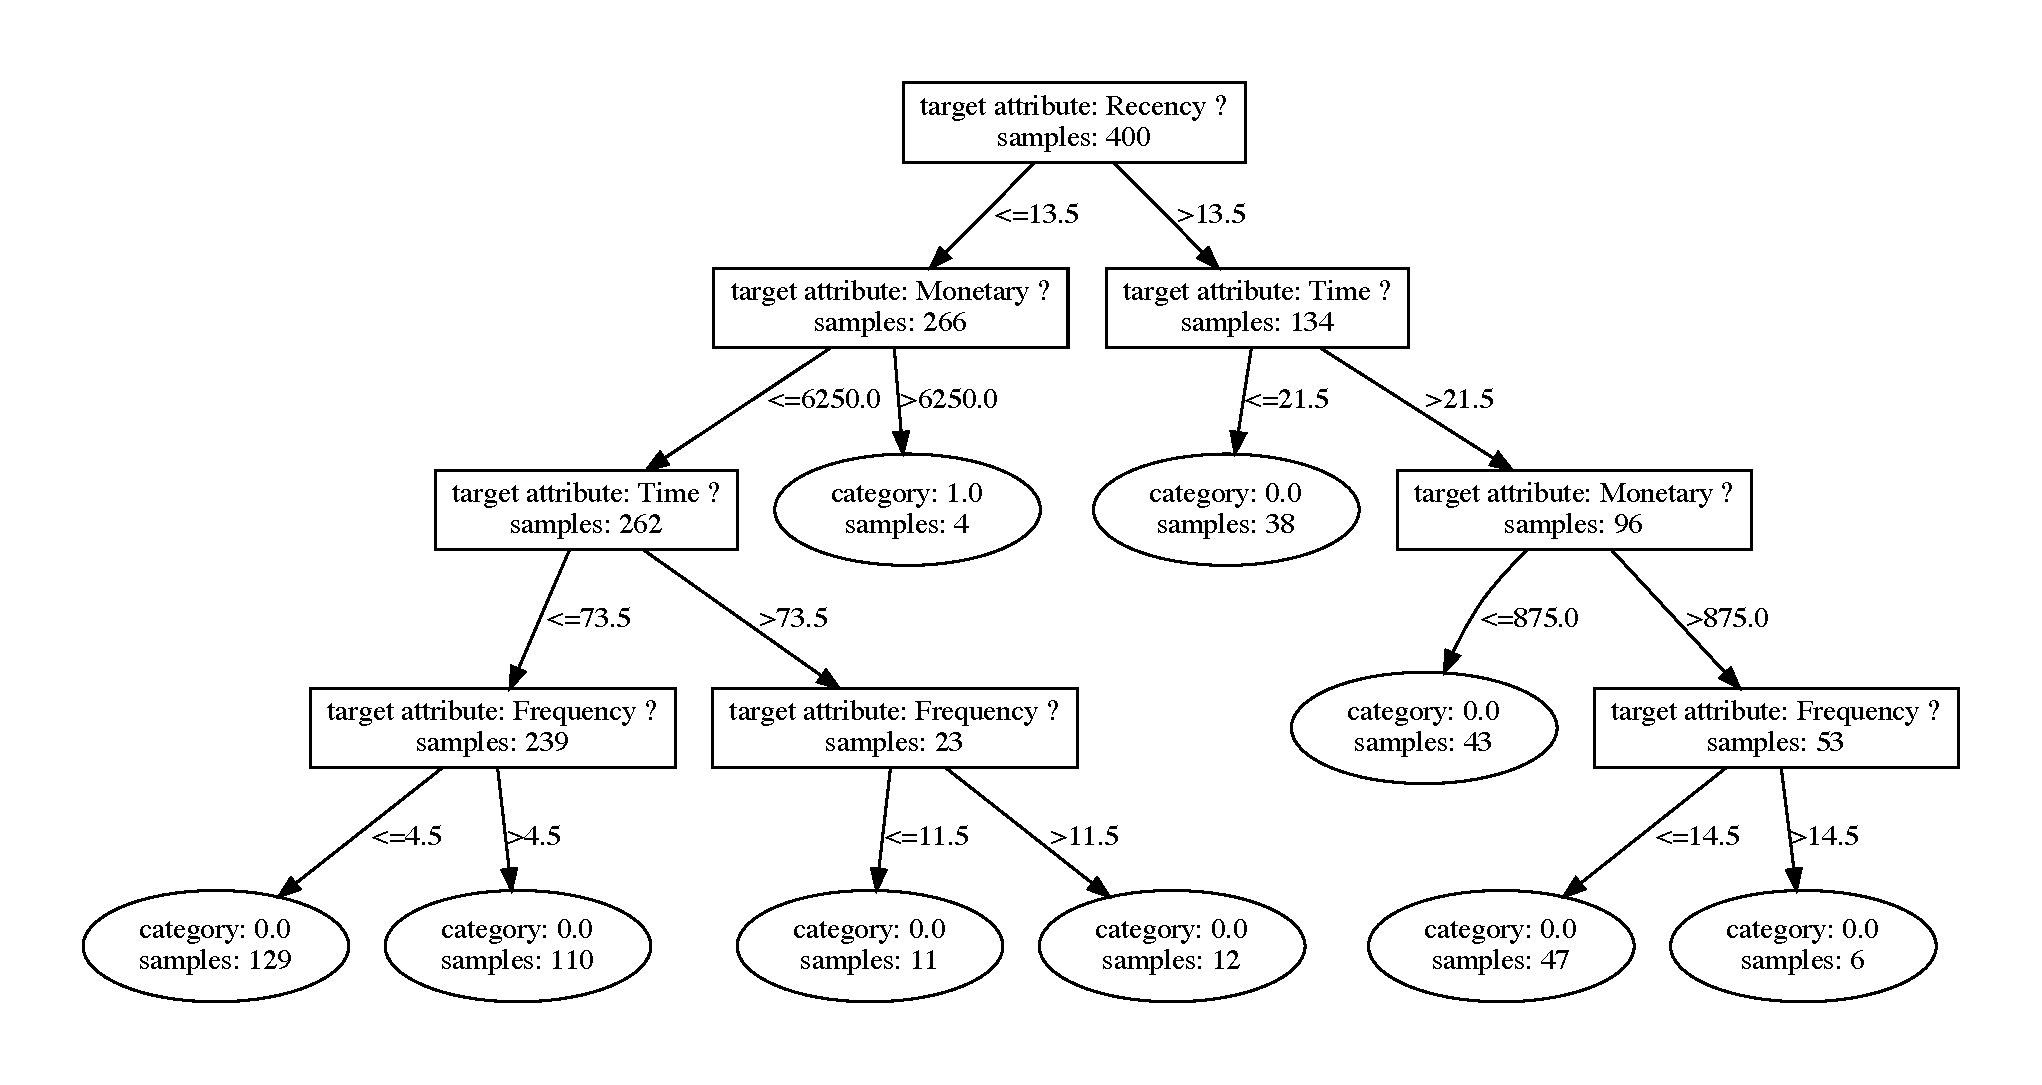
\includegraphics[width=0.48\textwidth]{img/RF_vis/test_3_random_decision_tree_0.pdf}
    }
    \subfigure[基学习器2/20]{
        \includegraphics[width=0.48\textwidth]{img/RF_vis/test_3_random_decision_tree_1.pdf}
    }
    \quad
    \subfigure[基学习器3/20]{
        \includegraphics[width=0.48\textwidth]{img/RF_vis/test_3_random_decision_tree_2.pdf}
    }
    \subfigure[基学习器4/20]{
        \includegraphics[width=0.48\textwidth]{img/RF_vis/test_3_random_decision_tree_3.pdf}
    }
    \quad
    \subfigure[基学习器5/20]{
        \includegraphics[width=0.48\textwidth]{img/RF_vis/test_3_random_decision_tree_4.pdf}
    }
    \subfigure[基学习器6/20]{
        \includegraphics[width=0.48\textwidth]{img/RF_vis/test_3_random_decision_tree_5.pdf}
    }
    \quad
    \subfigure[基学习器7/20]{
        \includegraphics[width=0.48\textwidth]{img/RF_vis/test_3_random_decision_tree_6.pdf}
    }
    \subfigure[基学习器8/20]{
        \includegraphics[width=0.48\textwidth]{img/RF_vis/test_3_random_decision_tree_7.pdf}
    }
    \quad
    \subfigure[基学习器9/20]{
        \includegraphics[width=0.48\textwidth]{img/RF_vis/test_3_random_decision_tree_8.pdf}
    }
    \subfigure[基学习器10/20]{
        \includegraphics[width=0.48\textwidth]{img/RF_vis/test_3_random_decision_tree_9.pdf}
    }
    \quad
    \subfigure[基学习器11/20]{
        \includegraphics[width=0.48\textwidth]{img/RF_vis/test_3_random_decision_tree_10.pdf}
    }
    \subfigure[基学习器12/20]{
        \includegraphics[width=0.48\textwidth]{img/RF_vis/test_3_random_decision_tree_11.pdf}
    }
    \caption{在UCI数据集上生成的随机森林可视化}
    \label{rf_uci_vis}
\end{figure}

\begin{figure}[htbp!]
    \centering 
    \subfigure[基学习器13/20]{
        \includegraphics[width=0.48\textwidth]{img/RF_vis/test_3_random_decision_tree_12.pdf}
    }
    \subfigure[基学习器14/20]{
        \includegraphics[width=0.48\textwidth]{img/RF_vis/test_3_random_decision_tree_13.pdf}
    }
    \quad
    \subfigure[基学习器15/20]{
        \includegraphics[width=0.48\textwidth]{img/RF_vis/test_3_random_decision_tree_14.pdf}
    }
    \subfigure[基学习器16/20]{
        \includegraphics[width=0.48\textwidth]{img/RF_vis/test_3_random_decision_tree_15.pdf}
    }
    \quad
    \subfigure[基学习器17/20]{
        \includegraphics[width=0.48\textwidth]{img/RF_vis/test_3_random_decision_tree_16.pdf}
    }
    \subfigure[基学习器18/20]{
        \includegraphics[width=0.48\textwidth]{img/RF_vis/test_3_random_decision_tree_17.pdf}
    }
    \quad
    \subfigure[基学习器19/20]{
        \includegraphics[width=0.48\textwidth]{img/RF_vis/test_3_random_decision_tree_18.pdf}
    }
    \subfigure[基学习器20/20]{
        \includegraphics[width=0.48\textwidth]{img/RF_vis/test_3_random_decision_tree_19.pdf}
    }
    \caption{在UCI数据集上生成的随机森林可视化(续表\ref{rf_uci_vis})}
    \label{rf_uci_vis_2}
\end{figure}

\subsubsection{性能测试实验}
在实验\ref{dt_perfor_compare}的基础上,又增加了随机森林的性能测试实验,
这里基学习器的数量设置为200,Bootstrap样本数量设置为和训练集样本的数量一致。
整合的结果见表\ref{rf_perfor_compare}。从中,可以看出,随机森林在UCI
公开数据集上性能相较于单个决策树算法,有了明显的提升。

\begin{table}[]
    \caption{随机森林在UCI数据集上分类性能比较}
    \label{rf_perfor_compare}
    \centering
    \begin{tabular}{ccc}
    \hline
    算法   & 准确率                  & F1                   \\ \hline
    随机猜测 & 0.474±0.051          & 0.207±0.056 \\ \hline
    ID3  & 0.544±0.129          & 0.307±0.0.056         \\
    C4.5 & 0.647±0.132          & 0.275±0.192          \\
    CART & 0.652±0.139  & 0.280±0.175    \\ \hline
    RF   & \textbf{0.715±0.114}   & \textbf{0.314±0.161}    \\ \hline
    \end{tabular}
\end{table}

\section{综合实验设计和分析}
这里将主要展现基于随机森林的献血招募模型的相关实验,主要按照由浅入深、
由内而外的顺序,依次对数据集、模型对超参数和模型性能对比三个
维度,进行详尽全面的分析。

\subsection{数据集分析}
首先,对经过特征提取的预处理操作后的训练数据,进行初步分析,
掌握其分布特征,为后续的随机森林的模型参数设置作一定的基础准备
工作。

这里主要给出12个维度特征的分布示意图,包含了各自的箱形图(Box-whisker Plot),
以及直方图(Histogram),并利用核密度估计(Kernel Density Estimation)
绘制出了变量的概率密度函数。整个方法背后主要的指导思想是Thirumalai等人
\cite{8245071}提出的利用统计学里的数据分析手段来分析肺癌患者的
特征。总的来看,每个维度的样本分布大致还是平衡的。

\begin{figure}[htbp!]
    \centering 
    \subfigure[箱形图]{
        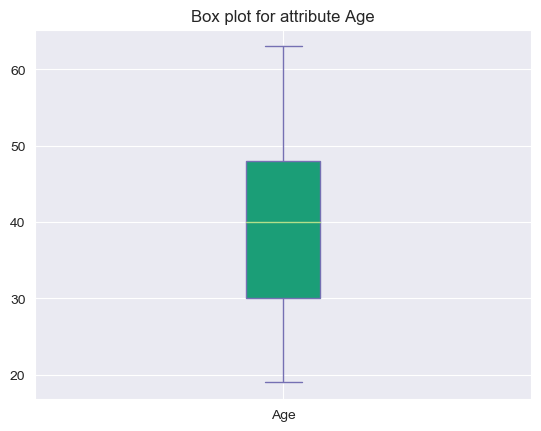
\includegraphics[width=0.44\textwidth]{img/data_vis/age.png}
    }
    \subfigure[直方图]{
        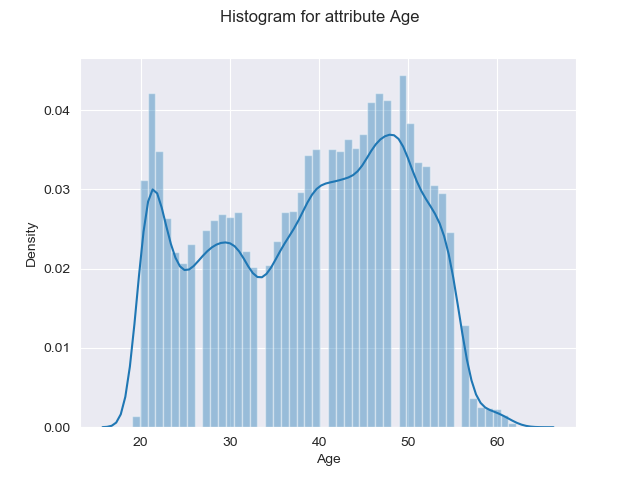
\includegraphics[width=0.44\textwidth]{img/data_vis/dis_Age.png}
    }
    \caption{样本\textbf{年龄}特征分布}
    \label{age_dis}
\end{figure}

\begin{figure}[htbp!]
    \centering 
    \subfigure[箱形图]{
        \includegraphics[width=0.44\textwidth]{img/data_vis/Sex.png}
    }
    \subfigure[直方图]{
        \includegraphics[width=0.44\textwidth]{img/data_vis/dis_Sex.png}
    }
    \caption{样本\textbf{性别}特征分布}
    \label{sex_dis}
\end{figure}

\begin{figure}[htbp!]
    \centering 
    \subfigure[箱形图]{
        \includegraphics[width=0.44\textwidth]{img/data_vis/Last_donation_volume.png}
    }
    \subfigure[直方图]{
        \includegraphics[width=0.44\textwidth]{img/data_vis/dis_Last_donation_volume.png}
    }
    \caption{样本\textbf{最近一次献血量}特征分布}
    \label{last_volume_dis}
\end{figure}

\begin{figure}[htbp!]
    \centering 
    \subfigure[箱形图]{
        \includegraphics[width=0.44\textwidth]{img/data_vis/Total_donation_volume.png}
    }
    \subfigure[直方图]{
        \includegraphics[width=0.44\textwidth]{img/data_vis/dis_Total_donation_volume.png}
    }
    \caption{样本\textbf{总献血量}特征分布}
    \label{total_volume_dis}
\end{figure}

\begin{figure}[htbp!]
    \centering 
    \subfigure[箱形图]{
        \includegraphics[width=0.44\textwidth]{img/data_vis/Total_number_of_donation.png}
    }
    \subfigure[直方图]{
        \includegraphics[width=0.44\textwidth]{img/data_vis/dis_Total_number_of_donation.png}
    }
    \caption{样本\textbf{献血次数}特征分布}
    \label{number_dis}
\end{figure}

\begin{figure}[htbp!]
    \centering 
    \subfigure[箱形图]{
        \includegraphics[width=0.44\textwidth]{img/data_vis/Last_time_eligibility.png}
    }
    \subfigure[直方图]{
        \includegraphics[width=0.44\textwidth]{img/data_vis/dis_Last_time_eligibility.png}
    }
    \caption{样本\textbf{上次献血是否合格}特征分布}
    \label{eligibility_dis}
\end{figure}

\begin{figure}[htbp!]
    \centering 
    \subfigure[箱形图]{
        \includegraphics[width=0.44\textwidth]{img/data_vis/Occupation.png}
    }
    \subfigure[直方图]{
        \includegraphics[width=0.44\textwidth]{img/data_vis/dis_Occupation.png}
    }
    \caption{样本\textbf{职业}特征分布}
    \label{occupation_dis}
\end{figure}

\begin{figure}[htbp!]
    \centering 
    \subfigure[箱形图]{
        \includegraphics[width=0.44\textwidth]{img/data_vis/Interval.png}
    }
    \subfigure[直方图]{
        \includegraphics[width=0.44\textwidth]{img/data_vis/dis_Interval.png}
    }
    \caption{样本\textbf{献血间隔}特征分布}
    \label{interval_dis}
\end{figure}

\begin{figure}[htbp!]
    \centering 
    \subfigure[箱形图]{
        \includegraphics[width=0.44\textwidth]{img/data_vis/Education.png}
    }
    \subfigure[直方图]{
        \includegraphics[width=0.44\textwidth]{img/data_vis/dis_Education.png}
    }
    \caption{样本\textbf{受教育程度}特征分布}
    \label{education_dis}
\end{figure}

\begin{figure}[htbp!]
    \centering 
    \subfigure[箱形图]{
        \includegraphics[width=0.44\textwidth]{img/data_vis/Neighbourhood.png}
    }
    \subfigure[直方图]{
        \includegraphics[width=0.44\textwidth]{img/data_vis/dis_Neighbourhood.png}
    }
    \caption{样本\textbf{居住情况}特征分布}
    \label{neighbourhood_dis}
\end{figure}

\begin{figure}[htbp!]
    \centering 
    \subfigure[箱形图]{
        \includegraphics[width=0.44\textwidth]{img/data_vis/Reaction.png}
    }
    \subfigure[直方图]{
        \includegraphics[width=0.44\textwidth]{img/data_vis/dis_Reaction.png}
    }
    \caption{样本\textbf{是否有献血反应}特征分布}
    \label{reaction_dis}
\end{figure}

\begin{figure}[htbp!]
    \centering 
    \subfigure[箱形图]{
        \includegraphics[width=0.44\textwidth]{img/data_vis/Frequency.png}
    }
    \subfigure[直方图]{
        \includegraphics[width=0.44\textwidth]{img/data_vis/dis_Frequency.png}
    }
    \caption{样本\textbf{献血频率}特征分布}
    \label{frequency_dis}
\end{figure}

\subsection{超参数分析}
\subsubsection{外部参数}
在模型的外部参数方面,对随机森林模型性能有显著影响的主要
是训练样本的数目。这里,针对训练样本的规模对随机森林性能
的影响,进行了细致全面的分析。

固定了随机森林的所有内部超参数(基分类器的数量固定为100),仅改变输入的训练样本数量,
得到的实验结果如\ref{hyper_training_data_oob}
和\ref{hyper_training_data_acc}所示。
横轴表示,给定一定数量的训练样本,
每次不断增加模型使用的训练样本的占比,观察OOB错误率和
测试集上的平均预测正确率(使用5折交叉验证)。可以发现,
整体来看,模型的性能随着训练数据的规模增大而提升,
在使用到训练数据集合的80\%之后,模型的性能趋于稳定。
并且,基于CART的随机森林在OOB错误率上相较于基于C4.5的随机森林
略有优势,而在预测精度方面,两者并无显著差别。

\begin{figure}[htbp!]
    \centering \includegraphics[width=0.6\textwidth]{img/hyperpara_out_oob.pdf} 
    \caption{训练集规模对OOB错误率的影响}
    \label{hyper_training_data_oob}
\end{figure}


\begin{figure}[htbp!]
    \centering \includegraphics[width=0.6\textwidth]{img/hyperpara_out_mean_acc.pdf} 
    \caption{训练集规模对预测精度的影响}
    \label{hyper_training_data_acc}
\end{figure}


\subsubsection{内部参数}
内部参数主要有三个:a)基分类器的数量,b)决策树生成算法和c)分裂节点时
选择特征的比例公式。

当基分类器的数目不断增加时,采取不同的决策树生成算法CART和C4.5,可以
得到结果如图\ref{hyper_ab_oob}和\ref{hyper_ab_acc}所示。
从中可以看出,横轴是基分类器的数目,大约在100之后,模型的性能趋于稳定。
并且C4.5算法和CART算法在OOB错误率上无明显差距,前者在预测精度上
略占优势。

\begin{figure}[htbp!]
    \centering \includegraphics[width=0.6\textwidth]{img/hyperpara_criterion_oob_2.pdf} 
    \caption{基分类器数目和决策树生成算法对OOB错误率的影响}
    \label{hyper_ab_oob}
\end{figure}


\begin{figure}[htbp!]
    \centering \includegraphics[width=0.6\textwidth]{img/hyperpara_criterion_mean_acc_2.pdf} 
    \caption{基分类器数目和决策树生成算法对预测精度的影响}
    \label{hyper_ab_acc}
\end{figure}

另一方面,当基分类器的数目不断增加时,在分裂节点时考虑不同的特征选取比例,
依据Wang等人的最新研究\cite{wang2020forest},一般采取三种选取方式。
假设$N$为当前节点中所有的特征数目,$M$为待选取的特征数目。那么$M$有三种
取值方式。$M=\sqrt{N}$,$M=\log _{2}{N}$和$M=N$。这样可以得到结果如图\ref{hyper_ac_oob}和\ref{hyper_ac_acc}所示。
从中可以看出,横轴是基分类器的数目,大约在100之后,模型的性能趋于稳定。
由于本数据集中特征数目只有12,所以无法看出$M=\sqrt{N}$和$M=\log _{2}{N}$
之间的差别。并且$M=N$选择比例和$M=\sqrt{N}$选择比例在OOB错误率上无明显差距,
前者在预测精度上略占优势。

\begin{figure}[htbp!]
    \centering \includegraphics[width=0.6\textwidth]{img/hyperpara_max_features_oob_2.pdf} 
    \caption{基分类器数目和节点分裂时特征选择比例对OOB错误率的影响}
    \label{hyper_ac_oob}
\end{figure}


\begin{figure}[htbp!]
    \centering \includegraphics[width=0.6\textwidth]{img/hyperpara_max_features_mean_acc_2.pdf} 
    \caption{基分类器数目和节点分裂时特征选择比例对预测精度的影响}
    \label{hyper_ac_acc}
\end{figure}

\subsection{模型性能分析}


经过上述的超参数分析,选择一组合适的超参数固定随机森林算法。
基分类器的数目设置为100,选择CART算法作为生成决策树的算法,
特征选择比例为$M=\sqrt{N}$。

首先将随机森林算法和基准单个的决策树算法以及其他常见的集成学习
算法做比较。得到的结果见表\ref{compare_ensemble},
对应的ROC曲线见\ref{roc_1}。
可以看出,在基分类器决策树的基础上,其它的集成学习
算法性能都有了明显的提升。由于引入了特征的随机选择,随机森林
算法比一般的Bagging+决策树的方法略有优势。此外,Boosting家族
的算法AdaBoost和Gradient Boosting性能差不多,略弱于随机森林。
原因主要在于:Boosting算法主要针对于高偏差(Bias)低方差(Variance)
的基分类器,Bagging算法则恰好相反,主要针对于低偏差(Bias)
高方差(Variance)的基分类器,决策树属于后者,所以随机森林的性能
会略有优势。

\begin{table}[]
    \caption{随机森林在真实数据集上性能比较(与其他集成学习算法比较)}
    \label{compare_ensemble}
    \centering
    \begin{tabular}{ccc}
    \hline
    算法                    & 准确率                  & F1          \\ \hline
    Decision Tree         & 0.929±0.042          & 0.731±0.596 \\ 
    Bagging+Decision Tree & 0.956±0.039          & 0.838±0.583 \\
    AdaBoost              & 0.950±0.032          & 0.821±0.221 \\
    Gradient Boosting     & 0.959±0.040          & 0.860±0.057 \\ \hline
    Random Forest         & \textbf{0.969±0.039} & \textbf{0.870±0.042} \\ \hline
    \end{tabular}
\end{table}

\begin{figure}[htbp!]
    \centering \includegraphics[width=1\textwidth]{img/intra_whole_roc.pdf} 
    \caption{表\ref{compare_ensemble}中对应算法的ROC曲线比较}
    \label{roc_1}
\end{figure}

更进一步地,为了探究除了集成学习以外的、其它常见的分类算法在该问题上的
性能,引入了SVM、KNN、Neural Network、SGD。将它们一一与随机森林进行
比较,得到的结果如表\ref{compare_other},对应的ROC曲线见图\ref{roc_2}。

从中可以看出,随机森林算法由于集成学习思想Bagging的加入,使得性能明显地
优于其他主流的非集成学习的分类算法。并且由于在特征提取的过程当中,加入了
许多专家知识,使得其他主流分类算法的性能仍然表现出色,准确率都在95\%左右。

\begin{table}[]
    \caption{随机森林在真实数据集上性能比较(与其他分类算法比较)}
    \label{compare_other}
    \centering
    \begin{tabular}{ccc}
    \hline
    算法             & 准确率                  & F1          \\ \hline
    SVM            & 0.952±0.042          & 0.450±0.129 \\
    KNN            & 0.943±0.004          & 0.691±0.031 \\
    Neural network & 0.941±0.002          & 0.738±0.008 \\
    SGD            & 0.952±0.142          & 0.860±0.057 \\ \hline
    Random Forest             & \textbf{0.969±0.039} & \textbf{0.930±0.042} \\ \hline
    \end{tabular}
\end{table}

\begin{figure}[htbp!]
    \centering \includegraphics[width=1\textwidth]{img/inter_whole_roc.pdf} 
    \caption{表\ref{compare_other}中对应算法的ROC曲线比较}
    \label{roc_2}
\end{figure}

\end{document}